\usetikzlibrary{arrows}
\usetikzlibrary{positioning}

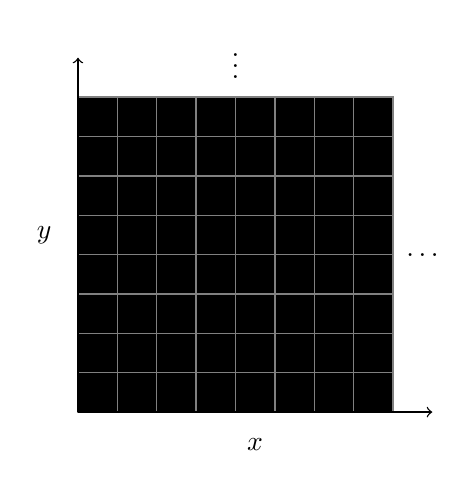
\begin{tikzpicture}[line width =0.5pt, scale=0.5]

\draw[gray] (0,0) grid (8,8);
\foreach \x in {0, 1, 2, 3, 4, 5, 6, 7}
    \foreach \y in {0, 1, 2, 3, 4, 5, 6, 7}
        \ifthenelse{\x<\y}{\def\col{white}}{\def\col{black}}
        \filldraw[fill=\col, draw=gray] (\x,\y) rectangle ++(1,1);

\draw[->] (0,0) -- (9,0) node[midway, below=6pt]{$x$};
\draw[->] (0,0) -- (0,9) node[midway, left=6pt]{$y$};
\node[] at (4,9){$\vdots$};
\node[] at (8.75,4){$\dots$};
\end{tikzpicture}